\documentclass{beamer}
\usetheme{metropolis}
\usepackage[polish]{babel}
\usepackage[utf8]{inputenc}
\usepackage{amsfonts}
\usepackage{indentfirst}
\usepackage[T1]{fontenc}
\usepackage{amsmath}
\usepackage{hyperref}
\usepackage{graphicx}
\usepackage{graphics}
\usepackage{subcaption}

\title{
Zaawansowane metody uczenia maszynowego
}
\subtitle{
Projekt 2
}
\author{
Mikołaj Małkiński
}
\institute{
Politechnika Warszawska \\
Wydział Matematyki i Nauk Informacyjnych
}
\date{\today}

\begin{document}

    \maketitle

    \begin{frame}{Spis treści}
        \setbeamertemplate{section in toc}[sections numbered]
        \tableofcontents[hideallsubsections]
    \end{frame}

    \section{Wstępna analiza danych}

    \begin{frame}
        \frametitle{Unikalność danych}
        \begin{figure}
            \centering
            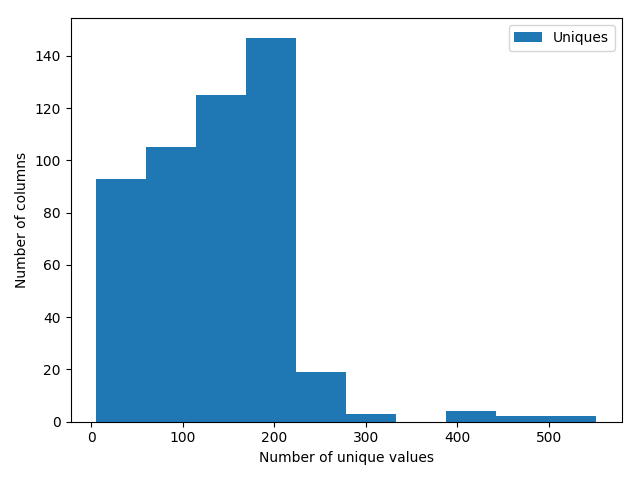
\includegraphics[width=0.8\linewidth]{../images/uniqueness-train.png}
            \caption{Unikalne wartości}
            \label{fig:uniqueness-train}
        \end{figure}
    \end{frame}

    \begin{frame}
        \frametitle{Rozkład cech z podziałem na zbiór}
        \begin{figure}[!h]
            \centering
            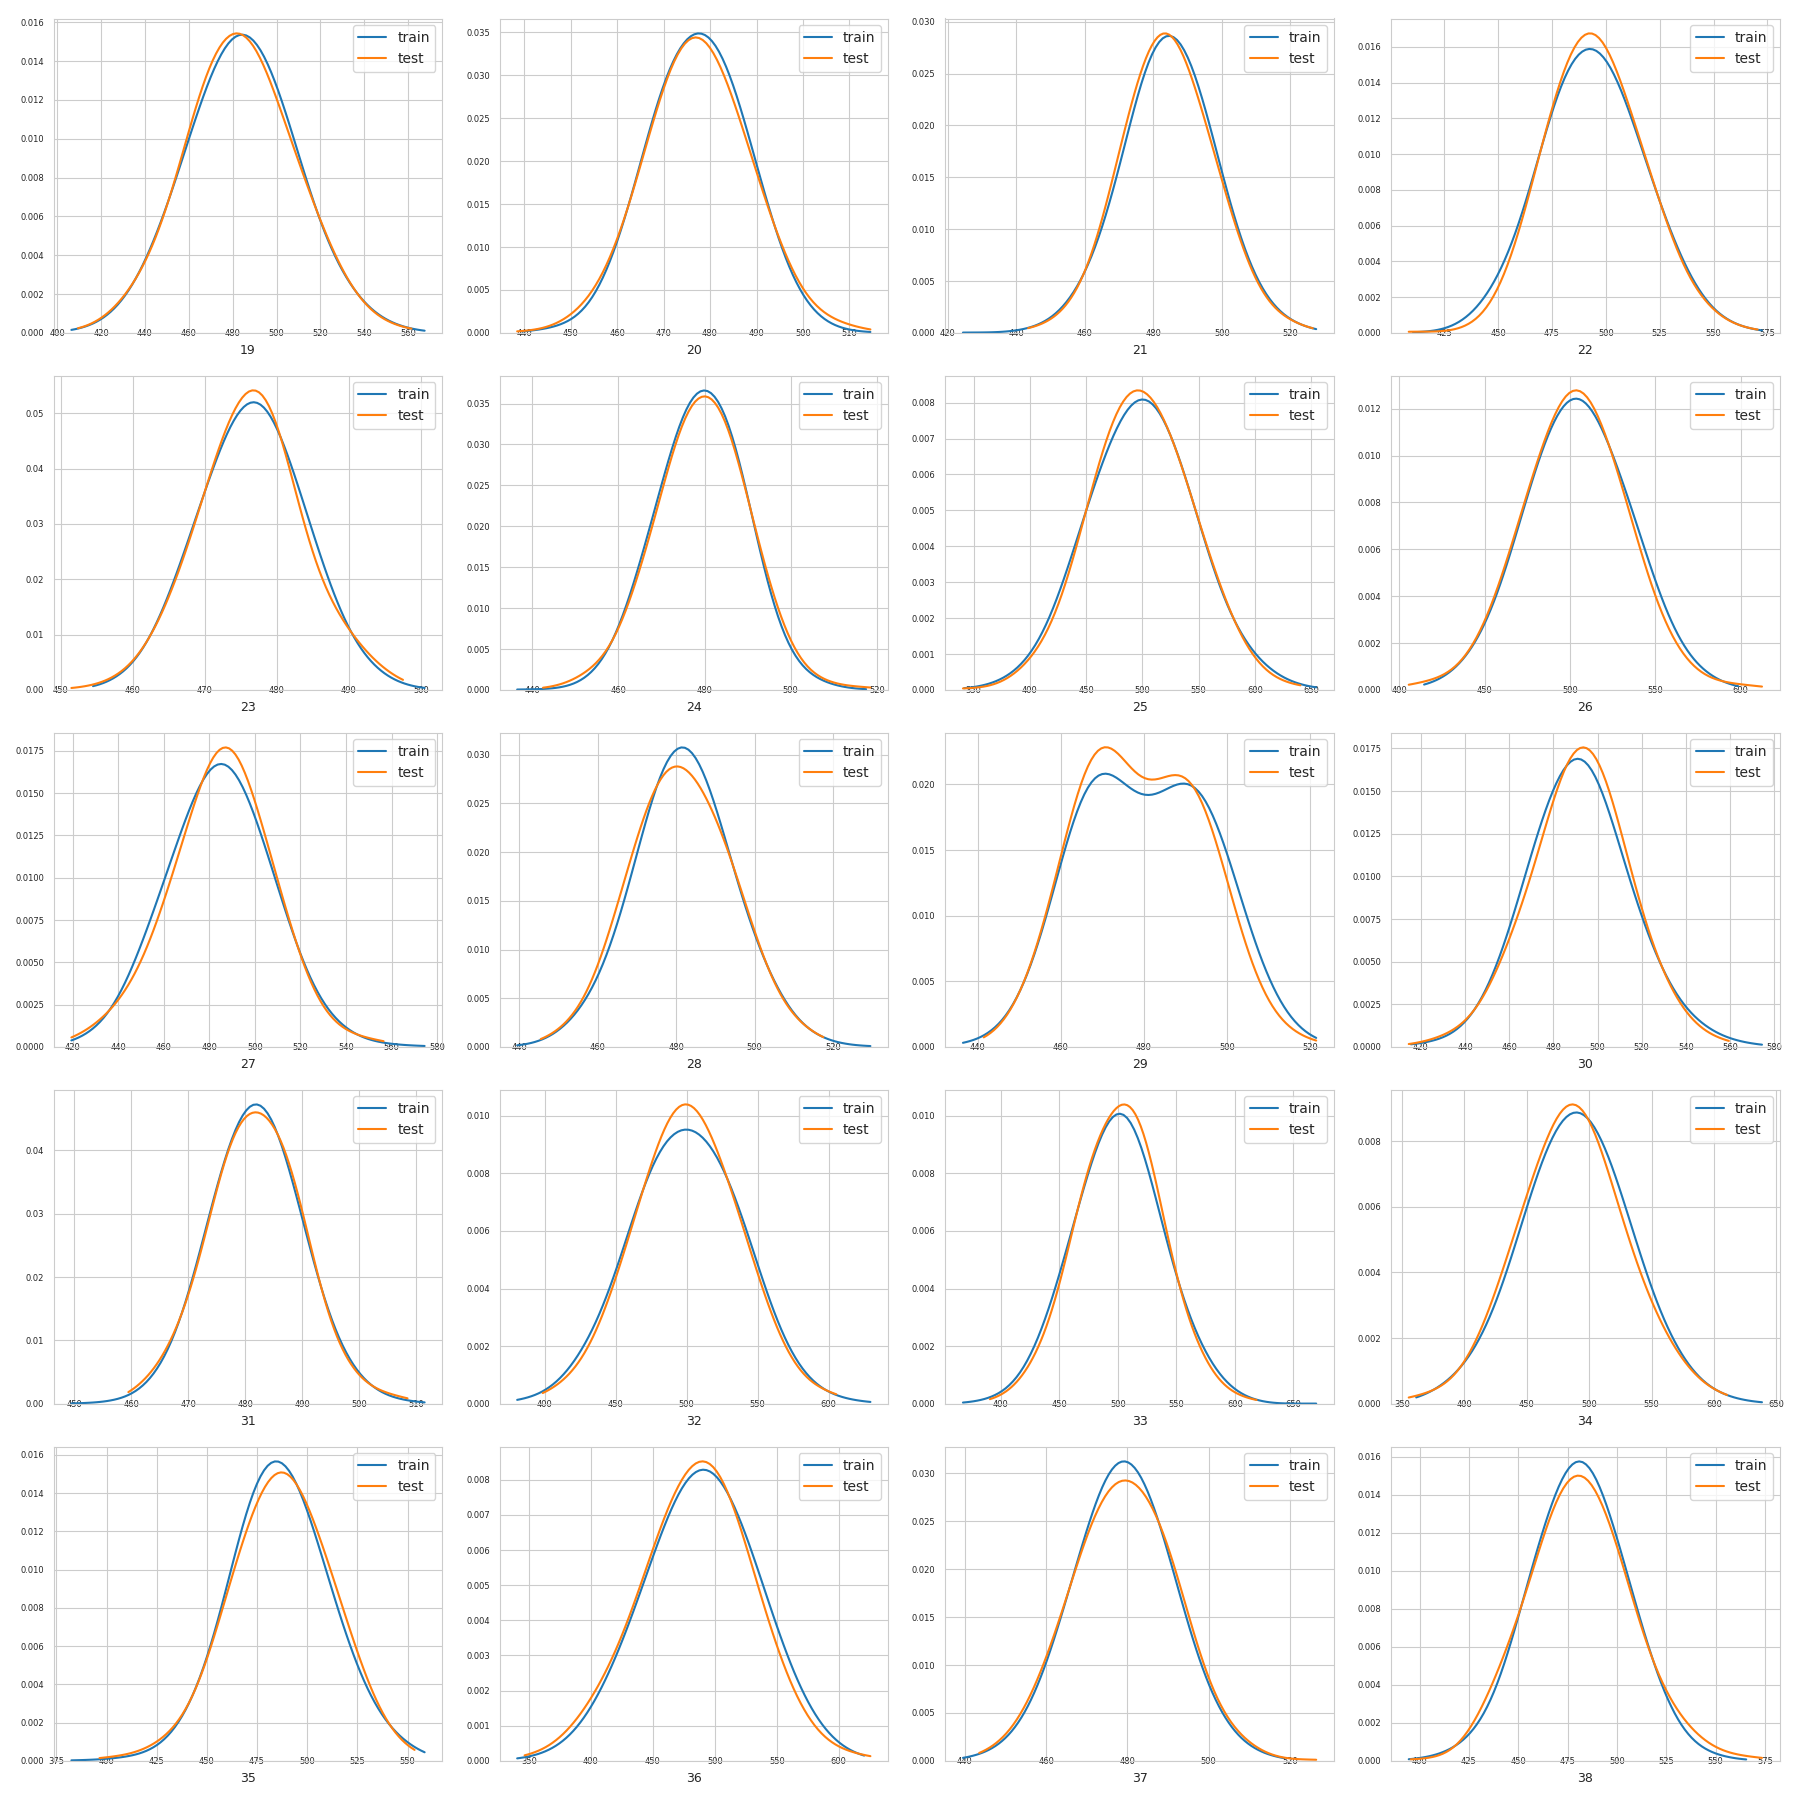
\includegraphics[width=0.7\textwidth]{../images/feature-distribution-dataset.png}
            \caption{Rozkład cech z podziałem na zbiór}
        \end{figure}
    \end{frame}

    \begin{frame}
        \frametitle{Rozkład cech z podziałem na klasę}
        \begin{figure}[!h]
            \centering
            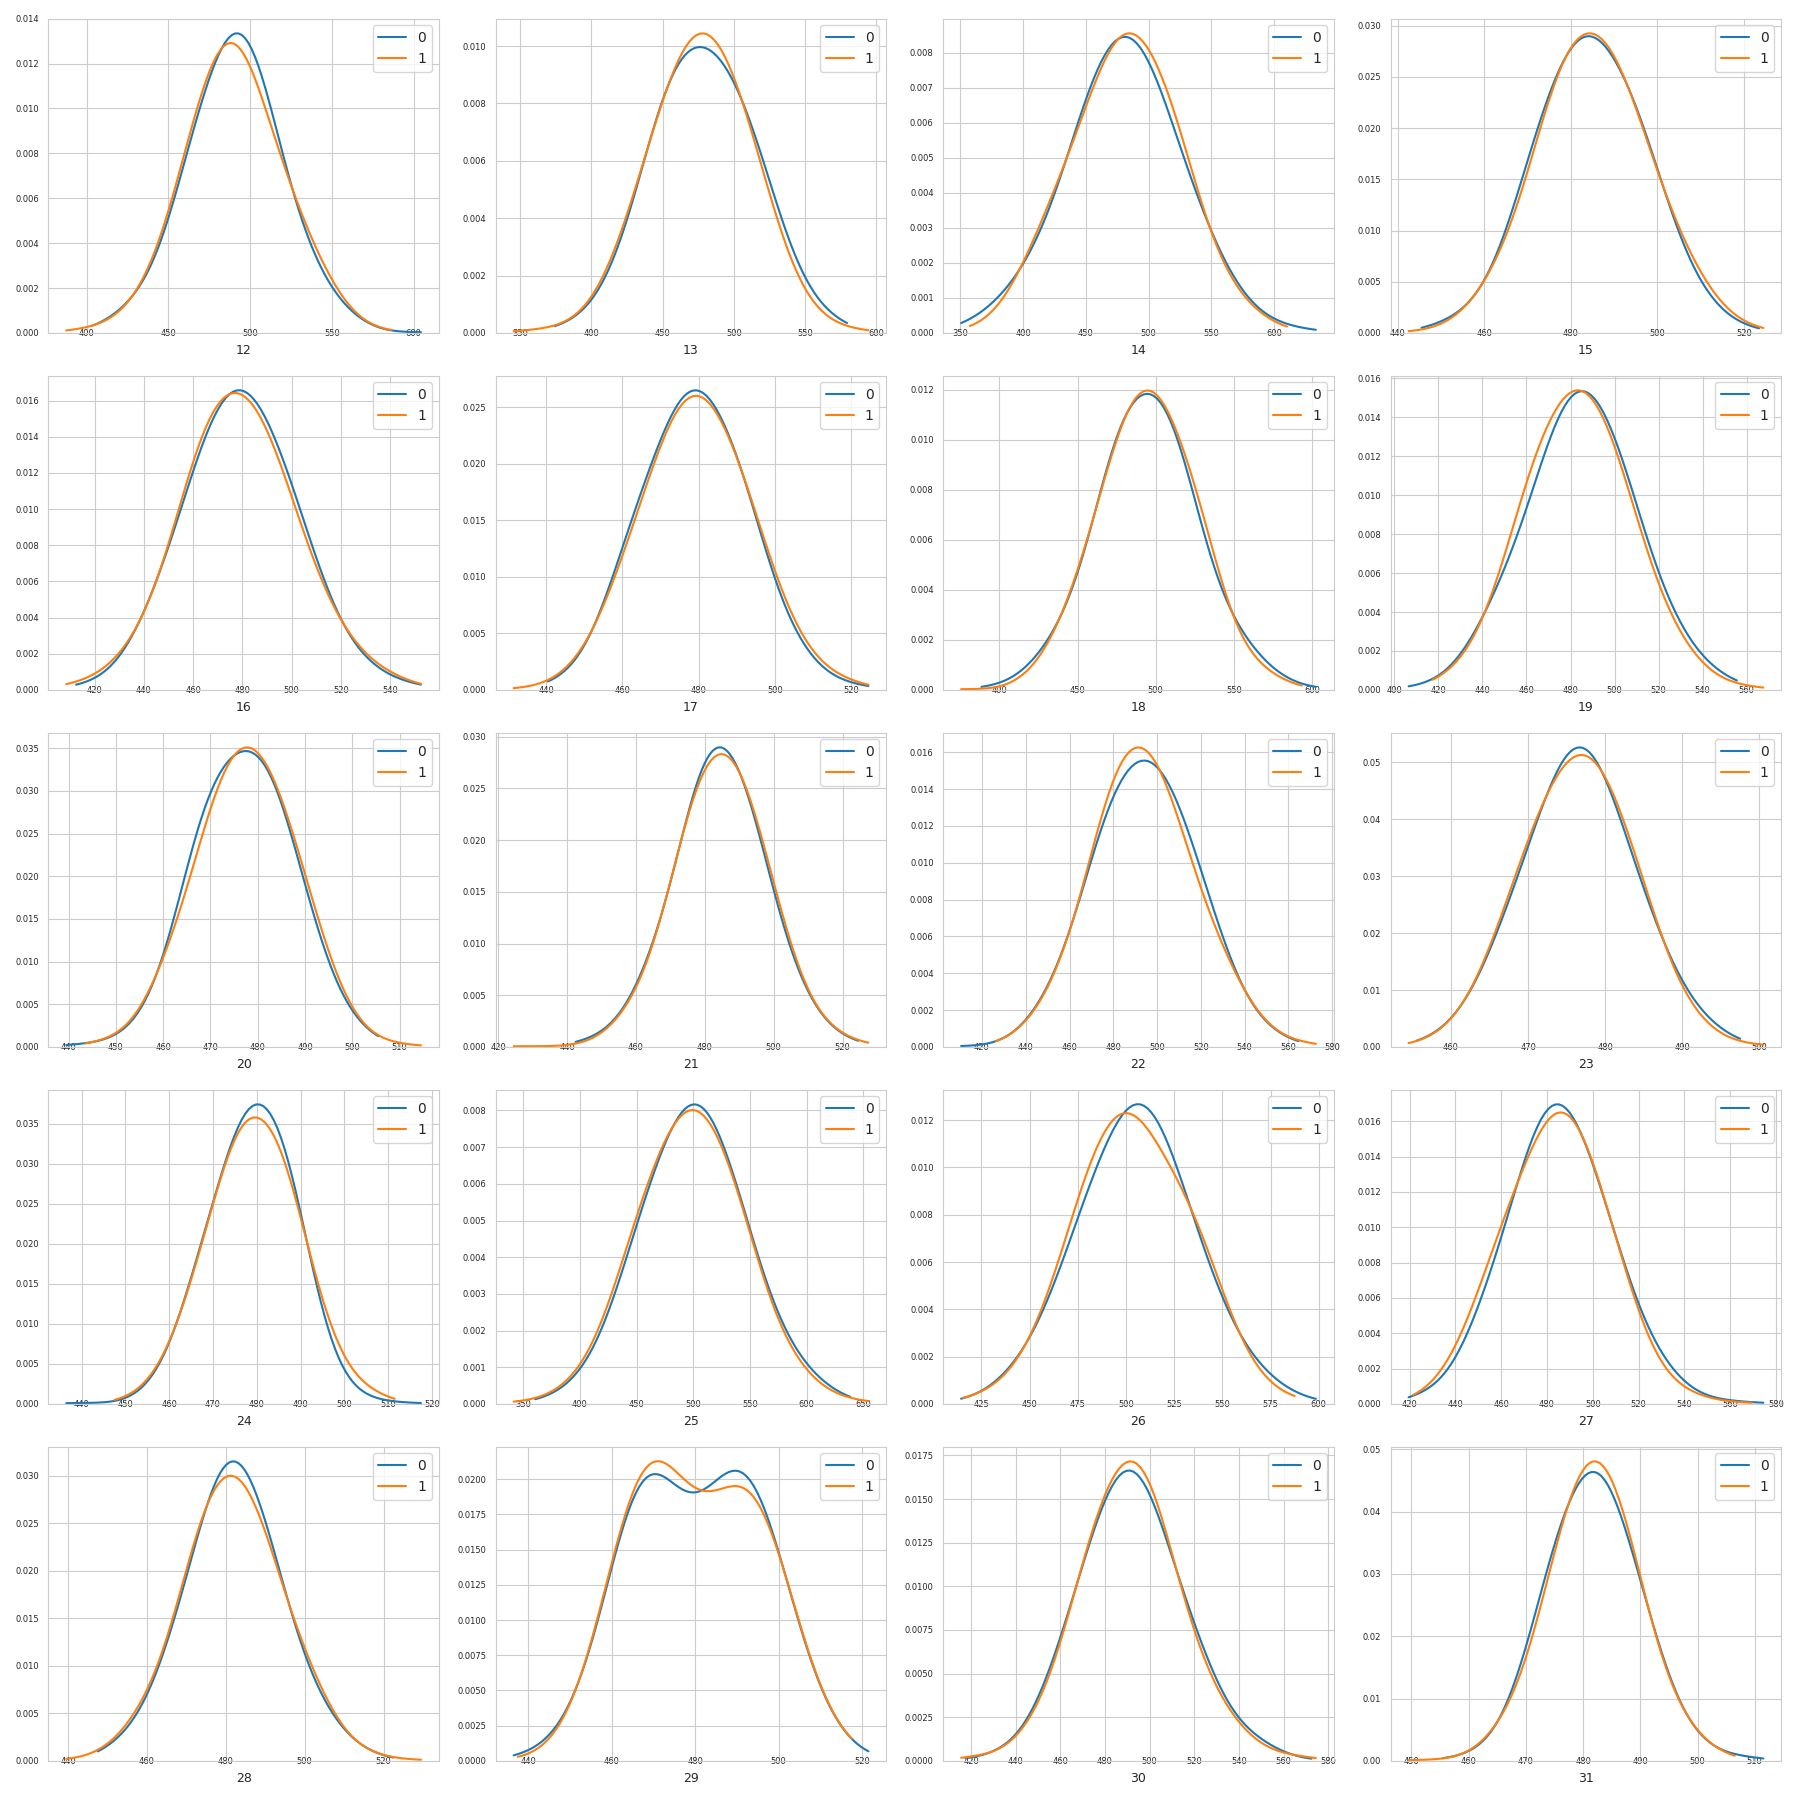
\includegraphics[width=0.7\textwidth]{../images/feature-distribution-label.png}
            \caption{Rozkład cech z podziałem na klasę}
        \end{figure}
    \end{frame}

    \section{Podstawowe modele w domyślnych konfiguracjach}

    \begin{frame}
        \frametitle{Wykorzystane klasyfikatory}
        \begin{itemize}
            \item XGBoost
            \item LightGBM
            \item AdaBoost
            \item GradientBoosting
            \item RandomForest
            \item ExtraTrees
        \end{itemize}
    \end{frame}

    \begin{frame}
        \frametitle{Krzywe ROC}
        \begin{figure}[!h]
            \centering
            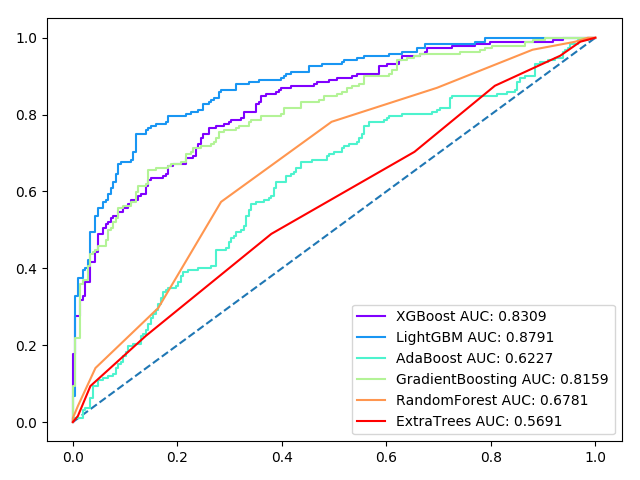
\includegraphics[width=0.8\linewidth]{../images/roc-comparison.png}
            \caption{Porównanie krzywych ROC podstawowych modeli klasyfikacyjnych}
            \label{fig:roc-comparison}
        \end{figure}
    \end{frame}

    \begin{frame}
        \frametitle{Metryki}
        \begin{table}
            \begin{tabular}{l|*{3}{c}}
                & AUC & Dokładność & Zbalansowana dokładność \\
                \hline
                XGBoost & 0.8309 & 0.7400 & 0.7390 \\
                LightGBM & \textbf{0.8791} & \textbf{0.8025} & \textbf{0.8023} \\
                AdaBoost & 0.6227 & 0.6125 & 0.6138 \\
                GradientBoosting & 0.8159 & 0.7275 & 0.7272 \\
                RandomForest & 0.6781 & 0.6475 & 0.6446 \\
                ExtraTrees & 0.5691 & 0.5575 & 0.5549 \\
            \end{tabular}
            \caption{Metryki podstawowych modeli klasyfikacyjnych}
            \label{tab:score-comparison-1}
        \end{table}
    \end{frame}

    \begin{frame}
        \frametitle{Metryki}
        \begin{table}
            \begin{tabular}{l|*{3}{c}}
                & F1 & Precyzja & Czułość \\
                \hline
                XGBoost & 0.7249 & 0.7366 & 0.7135 \\
                LightGBM & \textbf{0.7948} & \textbf{0.7927} & \textbf{0.7969} \\
                AdaBoost & 0.6154 & 0.5877 & 0.6458 \\
                GradientBoosting & 0.7169 & 0.7150 & 0.7188 \\
                RandomForest & 0.6094 & 0.6509 & 0.5729 \\
                ExtraTrees & 0.5151 & 0.5434 & 0.4896 \\
            \end{tabular}
            \caption{Metryki podstawowych modeli klasyfikacyjnych}
            \label{tab:score-comparison-2}
        \end{table}
    \end{frame}

    \section{Wybór cech}

    \begin{frame}
        \frametitle{Macierz korelacji}
        Ważne cechy: 476, 242, 129, 106, 49, 379.
        \begin{figure}
            \centering
            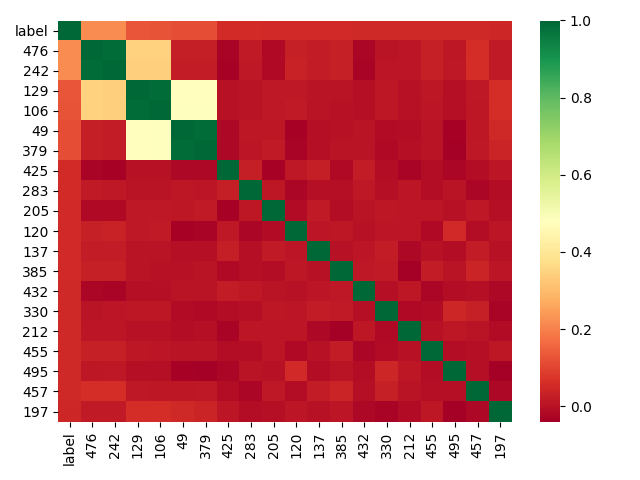
\includegraphics[width=0.8\linewidth]{../images/correlation-matrix.png}
            \caption{Macierz korelacji ograniczona do 20 największych wartości}
            \label{fig:correlation-matrix}
        \end{figure}
    \end{frame}

    \begin{frame}
        \frametitle{Analiza jednowymiarowa}
        Ponownie wyróżnione cechy: 476, 242, 106, 129, 49, 379.

        Nowe cechy: 337, 339, 443, 473, 454.
        \begin{figure}
            \centering
            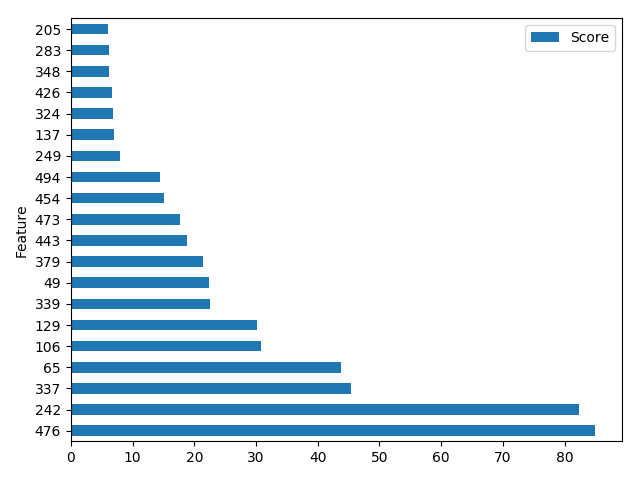
\includegraphics[width=0.65\linewidth]{../images/univariate-selection.png}
            \caption{20 największych wartości otrzymanych za pomocą testu ANOVA}
            \label{fig:univariate-selection}
        \end{figure}
    \end{frame}

    \begin{frame}
        \frametitle{Rekurencyjna eliminacja cech - LightGBM}
        Wybrane cechy: \textbf{106}, 154, 319, \textbf{337}, \textbf{379}, \textbf{443}, \textbf{454}.
        \begin{figure}[h!]
            \centering
            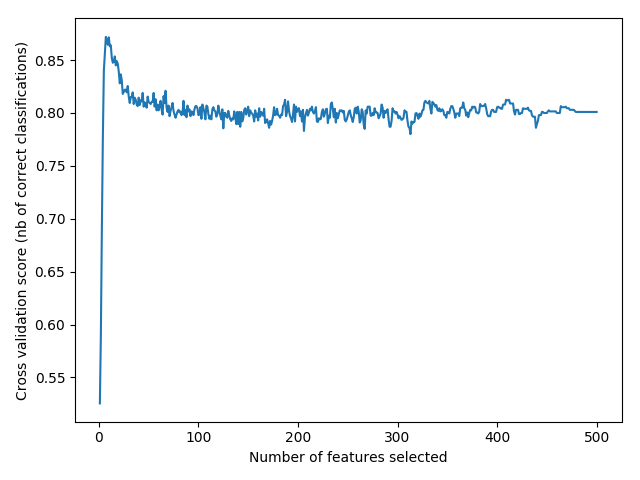
\includegraphics[width=0.75\linewidth]{../images/lightgbm-rfe-cv.png}
            \caption{Zbalansowana dokładność w zależności od liczby zmiennych}
            \label{fig:rfe-cv-lightgbm}
        \end{figure}
    \end{frame}

    \begin{frame}
        \frametitle{Rekurencyjna eliminacja cech - XGBoost}
        Wybrane cechy: 29, 49, \textbf{106}, 154, 242, 282, 319, \textbf{339}, \textbf{379}, \textbf{443}, 452, \textbf{473}, 476.
        \begin{figure}[h!]
            \centering
            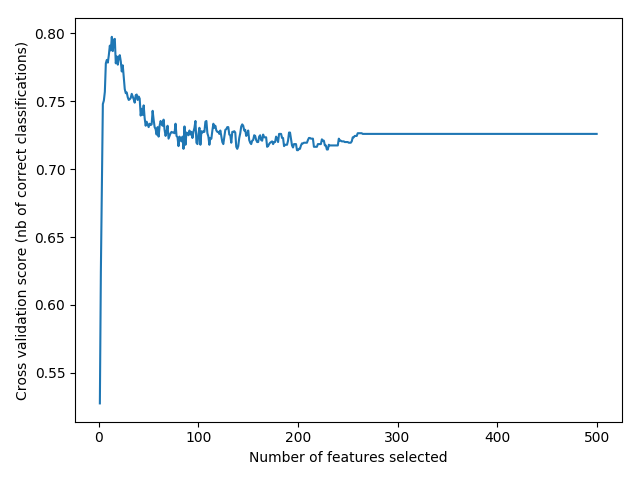
\includegraphics[width=0.75\linewidth]{../images/xgboost-rfe-cv.png}
            \caption{Zbalansowana dokładność w zależności od liczby zmiennych}
            \label{fig:rfe-cv-xgboost}
        \end{figure}
    \end{frame}

    \section{Dobór hiperparametrów}

    \begin{frame}
        \frametitle{Dobór hiperparametrów}
        \begin{itemize}
            \item Grid search
            \item 5-krotna kroswalidacja
            \item Maksymalizacja zbalansowanej dokładności
            \item Trening tylko na cechach wybranych przez dany model
            \item LightGBM - 87.2\%
            \item XGBoost - 85.9\%
        \end{itemize}
    \end{frame}

    \begin{frame}[standout]
        \centering
        Dziękuję za uwagę
    \end{frame}

\end{document}
